\subsubsection{Introducción}
\label{sec:core-service-introduction}

El \textit{core service} es el servicio backend encargado de coordinar las solicitudes
de los clientes, los servidores (\textit{world service}) y los almacenamientos (\textit{buckets}).
Este servicio posee diferentes módulos estructurados en carpetas. Los cuales son:

\begin{itemize}
    \item \underline{\textit{Assets service}}: Gestión y almacenamiento de los \textit{assets} de los mundos.
    \item \underline{\textit{Authentication service}}: Creación y login de los clientes.
    \item \underline{\textit{Exports service}}: Manejo de las versiones del \textit{game} y del \textit{world editor}.
    \item \underline{\textit{Payment service}}: Compra de gemas y manejo de suscripciones.
    \item \underline{\textit{Players service}}: Gestión de los nombres y \textit{skins} de los jugadores.
    \item \underline{\textit{World service}}: Gestión y publicación de los mundos.
\end{itemize}

Cada uno de ellos puede estar estructurado en más carpetas que separan subservicios; por ejemplo, \textit{assets service}
se divide en cada uno de sus \textit{assets}, o \textit{payment service} entre gemas y suscripciones. Sin embargo, todos
tienen en común la forma en que se desarrollan.
\vspace{0.25cm}

\begin{figure}[H]
    \centering
    \begin{adjustbox}{width=\textwidth, center}
        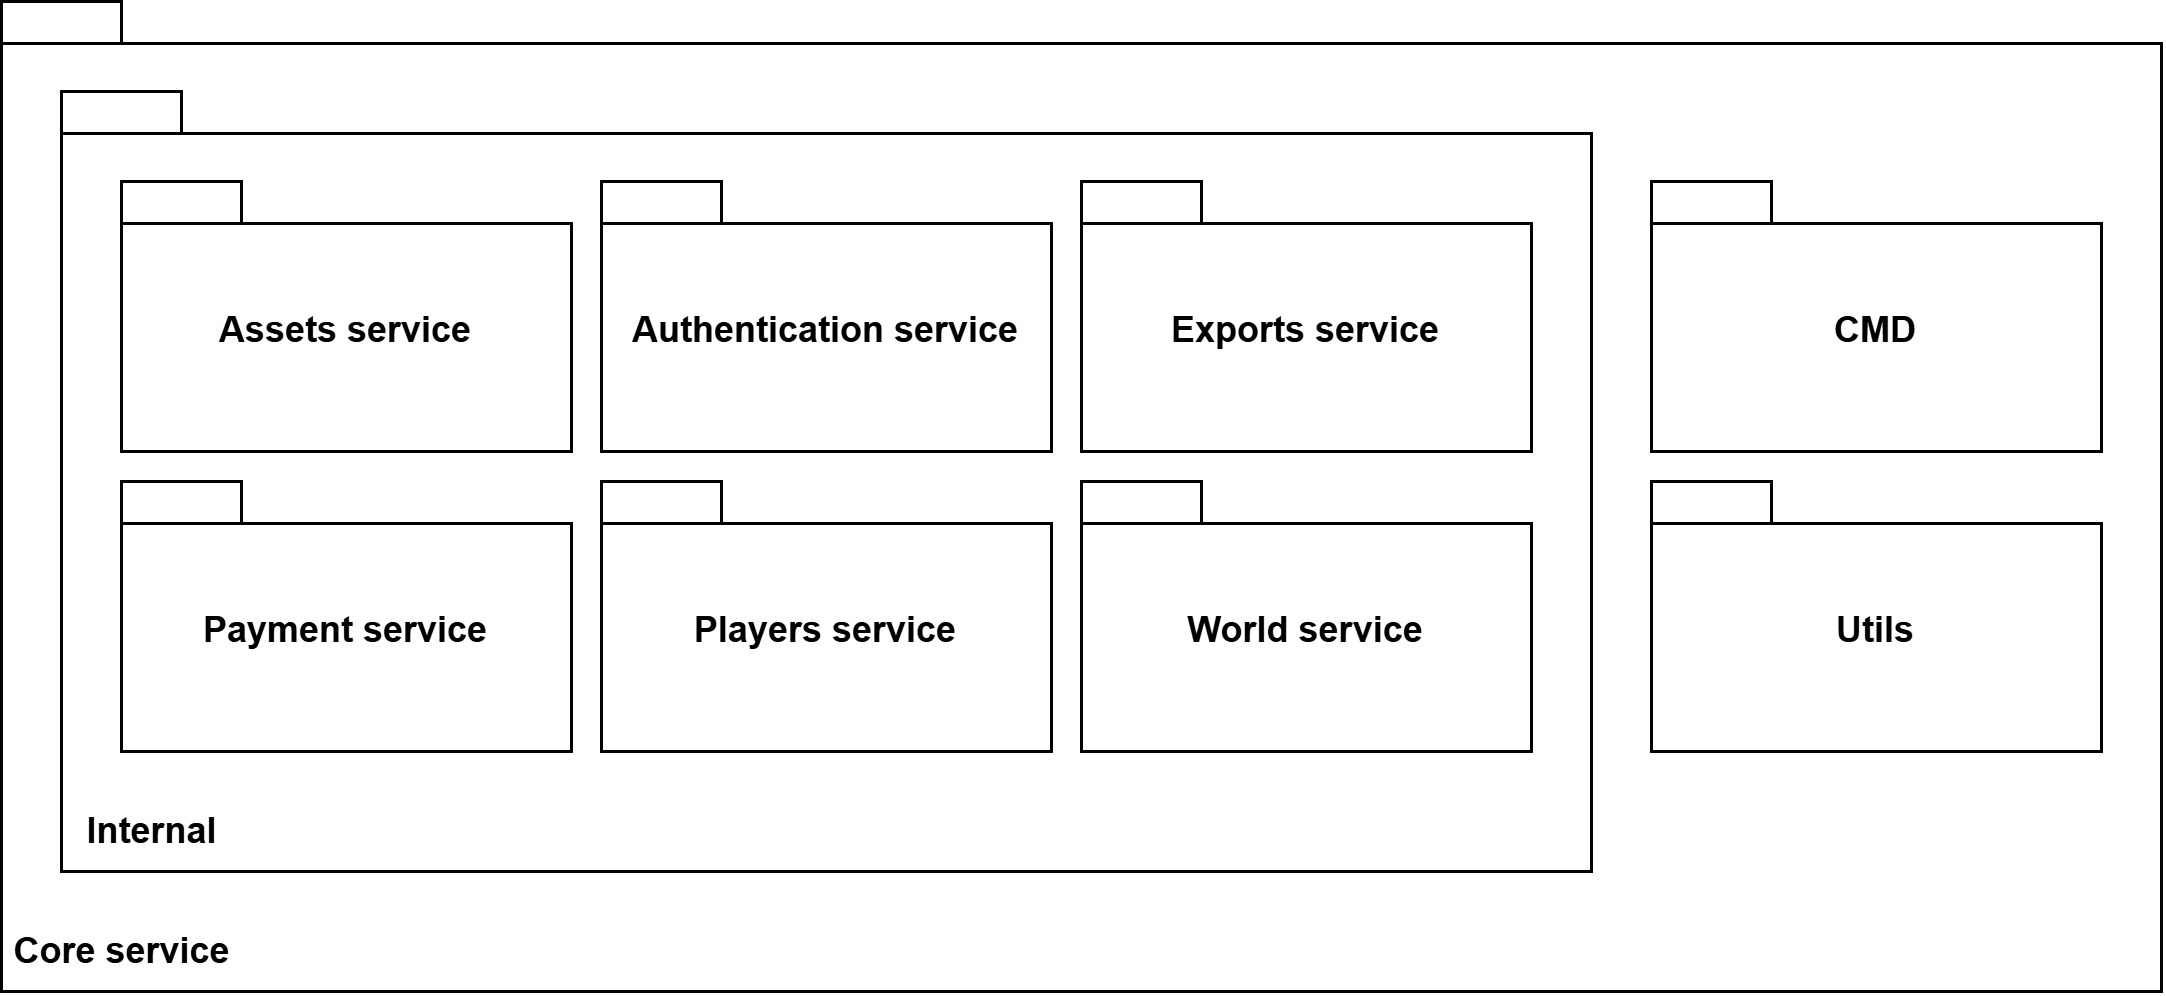
\includegraphics{img/09-technical-details/core-service/core-service-package.jpg}
    \end{adjustbox}
    \caption{Diagrama de paquetes del \textit{core service}.}    \label{fig:core-service-package}
\end{figure}

Todos se estructuran en diferentes capas o \textit{layers}; cada capa tiene un nivel de responsabilidad distinto.
La primera es el \textit{router}; ahí se hacen las definiciones de todas las rutas que tendrá cada uno de los servicios,
allí se crean las diferentes capas y se inyectan sus dependencias. 
\vspace{0.25cm}

\begin{figure}[H]
    \centering
    \begin{adjustbox}{width=0.3\textwidth, center}
        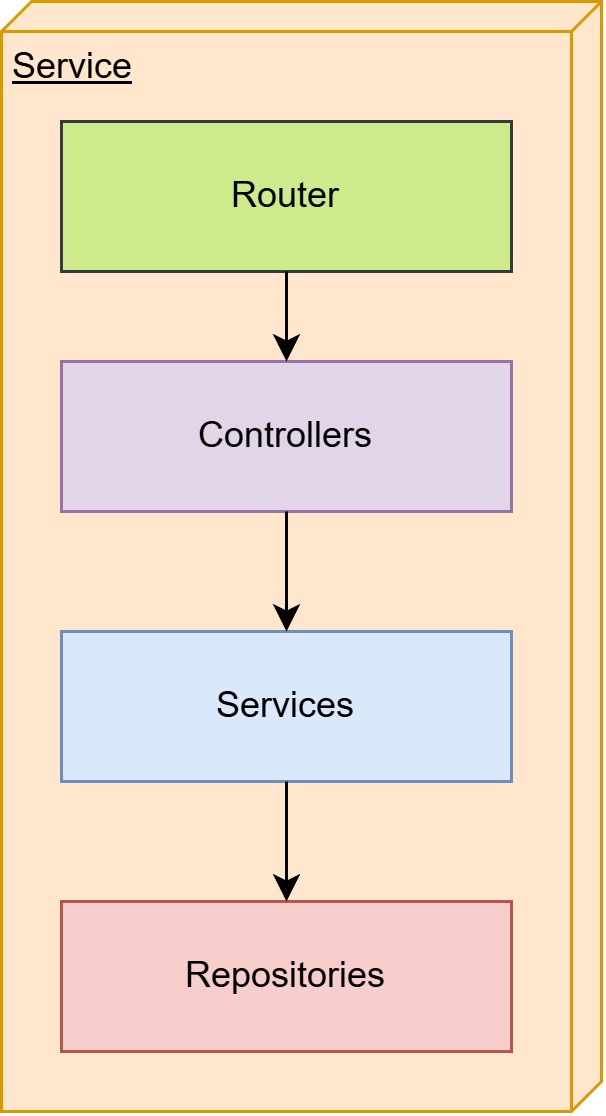
\includegraphics{img/09-technical-details/core-service/service-layers.jpg}
    \end{adjustbox}
    \caption{Diagrama donde se ven las capas (o \textit{layers}) de un servicio.}    \label{fig:service-layers}
\end{figure}

La segunda capa es el \textit{controller}; ahí se realiza el manejo de la petición HTTP para transformarla al lenguaje 
de negocio de la siguiente capa, \textit{service}, donde se realizan las operaciones propias del modelo de negocio. Por 
último, existe la capa de \textit{repository}, donde ocurre la comunicación con las bases de datos. Por otro lado, existe una 
carpeta de \textit{utils}, donde hay dependencias como el \textit{logger}, el manejo de contraseñas, la comunicación con 
el servicio de correo, la creación de los \textit{JWT}, entre otras cosas.
\vspace{0.25cm}
